\chapter{Éthique de la modélisation des dommages}
\label{chapter:ethique}
\newrefsegment

\PEEL{Les modélisateur.ices ont une responsabilité vis à vis de ce que leurs modèles produisent. }{Fournissez des preuves, des données ou des citations qui soutiennent votre point.}{Expliquez en quoi les preuves que vous avez fournies sont pertinentes et comment elles appuient votre point.}{Faites le lien avec le sujet principal ou avec la section suivante de votre mémoire.}


\chapterabstract{Nous avons identifié dans le chapitre \ref{chapter:modelisation} que les choix éthiques implicites ou explicites réalisés par les modélisateurs ont un impact sur le niveau de dommage dont l'amplitude est comparable à celle d'autres facteurs. Dans ce chapitre, nous explorons les enjeux éthiques que ce constat pose. Nous présentons les notions d'éthique procédurale, intrinsèque et extrinsèque. Nous montrons ensuite à travers les écrits de Longino, que la modélisation est fortement porteuse de valeurs. Nous nous interrogeons finalement sur la responsabilité qu'on les modélisateurs des effets de leurs résultats sur les politiques publiques. Nous avançons qu'il est essentiel que les hypothèses normatives soient plus clairement énoncées et qu'elles peuvent remettrent en cause la pertinence des modèles. Cependant, ces hypothèses ne semblent pas représenter de \emph{doute normativement innaproprié}.}

\newpage


Les modèles intégrés sont dans une position ambivalente : outils techniques complexes et abstraits, ils sont pourtant utilisés par des utilisateurs variés pour produire des décisions très concrètes. Cette tension est particulièrement claire dans le cas des fonctions de dommage. Comme nous avons pu le voir dans la partie précédente, les résultats qu'elles produisent sont très sensibles aux différentes hypothèses normatives sur lesquelles elles sont construites. Ainsi, la modélisation apparait empreinte de questions éthiques essentielles. 

Dans cette partie, nous reviendrons sur plusieurs points de tension, que nous éclairerons à l'aide de textes épistémologiques. 

Notre question de recherche principale sera la suivante : \textit{comment les systèmes normatifs des chercheurs transparaissent-ils dans les modèles ?}

Nous suivrons trois objectifs. D'abord, présenter des outils épistémologiques qui permettent d'éclairer ces questions. Ensuite, de présenter des points particuliers des modèles qui nous semblent porteurs d'enjeux éthiques, d'une manière qui se veut le plus proche possible du fonctionnement concret du modèle. Enfin, de croiser les deux approches pour proposer une lecture pratique de l'éthique de la modélisation des dommages. 

Dans un premier temps, nous présenterons le cadre conceptuel de Tuana, qui permet de décomposer en trois sphères les enjeux éthiques liés à la recherche. Nous discuterons ensuite de l'idée selon laquelle la modélisation des dommages impose une grille de lecture particulière, socialement, épistémologiquement et historiquement située, et cadre ainsi le débat sur l'action climatique. Enfin, nous aborderons la question de la responsabilité des chercheurs quant aux produits de leur recherche, notamment à travers le concept de doute normativement inapproprié. 





\cite{schienke_intrinsic_2011} => sur l'éthique intrinsèque dans les IAMs
\cite{weitzman_modeling_2009} => sur les événements non-linéaires



\section{Les trois niveaux de l'éthique et la responsabilité du modélisateur}

Cette section pose plusieurs questions quant à la place de la technique et de la modélisation dans la cité. 

Elle s'appuie notamment sur \cite{jonas_principe_2008} et \cite{edwards_vast_2013}, ainsi que sur la classification des enjeux éthiques de \cite{tuana_leading_2010}.


Comme nous l'avons vu précédemment, le processus de modélisation est avant tout un processus de sélection de ce qui est représenté et ce qui ne l'est pas, et de décision de la manière de le représenter. Comme nous le verrons dans le chapitre \ref{chapter:socio}, l'imperfection et la partialité des modèles est souvent assumée, voire revendiquée par les équipes de modélisation. Elle s'accompagne souvent d'une tentative de dé-responsabilisation de l'équipe de modélisation. Celle-ci prend généralement la forme suivante : 

\begin{authoredquote}
    Les résultats des modèles sont valables uniquement sous les conditions (nombreuses et irréalistes) dans lesquelles il a été conçu. On ne peut donc pas extrapoler les résultats, ou faire dire au modèle autre chose que ce qu'il veut dire. 
\end{authoredquote}

Pourtant, les résultats des modèles sont utilisés de manière large, notamment pour prendre des décisions de politique publique, y compris par des personnes n'ayant pas de compétence spécifique en modélisation, ni de connaissance particulière des modèles utilisés pour produire les connaissances qu'elles utilisent. Il y a donc un paradoxe : d'une part, l'idéal d'une compréhension fine des hypothèses de la modélisation, qui permet d'être conscient des choix de modélisation et de leurs implications. Cet idéal protège la responsabilité du modélisateur : en effet, les hypothèses ayant été clairement formulées, l'utilisateur final devient responsable de sa propre interprétation. Celle-ci se fait en accord avec les hypothèses énoncées, que l'utilisateur final fait sienne. D'autre part, il est difficile de comprendre un modèle pour plusieurs raisons : technique (les logiciels ne sont pas/plus accessibles), légales (le code source n'est pas accessible librement), capacitaires (les codes sources sont difficiles à interpréter, surtout si on n'est pas familier du langage utilisé), théoriques (les modèles intégrés font appel à des concepts issus de nombreuses disciplines). Cette difficulté à comprendre les modèles font que les résultats sont \textit{de facto} souvent interprétés dans l'état dans lequel ils sont délivrés, sans la contextualisation permise par le code. Dès lors, le choix des hypothèses est invisibilisé, et la responsabilité du modélisateur peut s'étendre jusqu'à l'interprétation du modèle, voire jusqu'aux conséquences de cette interprétation. \\

Pour éclairer ce paradoxe, nous allons nous intéresser aux dimensions éthiques de la modélisation. Pour cela, nous allons nous appuyer sur les travaux de Tuana, qui a cherché à développer un cadre conceptuel de l'éthique dans la recherche, et qu'elle a adapté spécifiquement au cas de la modélisation intégrée. \\

Elle développe trois dimensions éthiques de la recherche scientifique : l'éthique procédurale, l'éthique intrinsèque et l'éthique extrinsèque. 

\begin{figure}
    \centering

    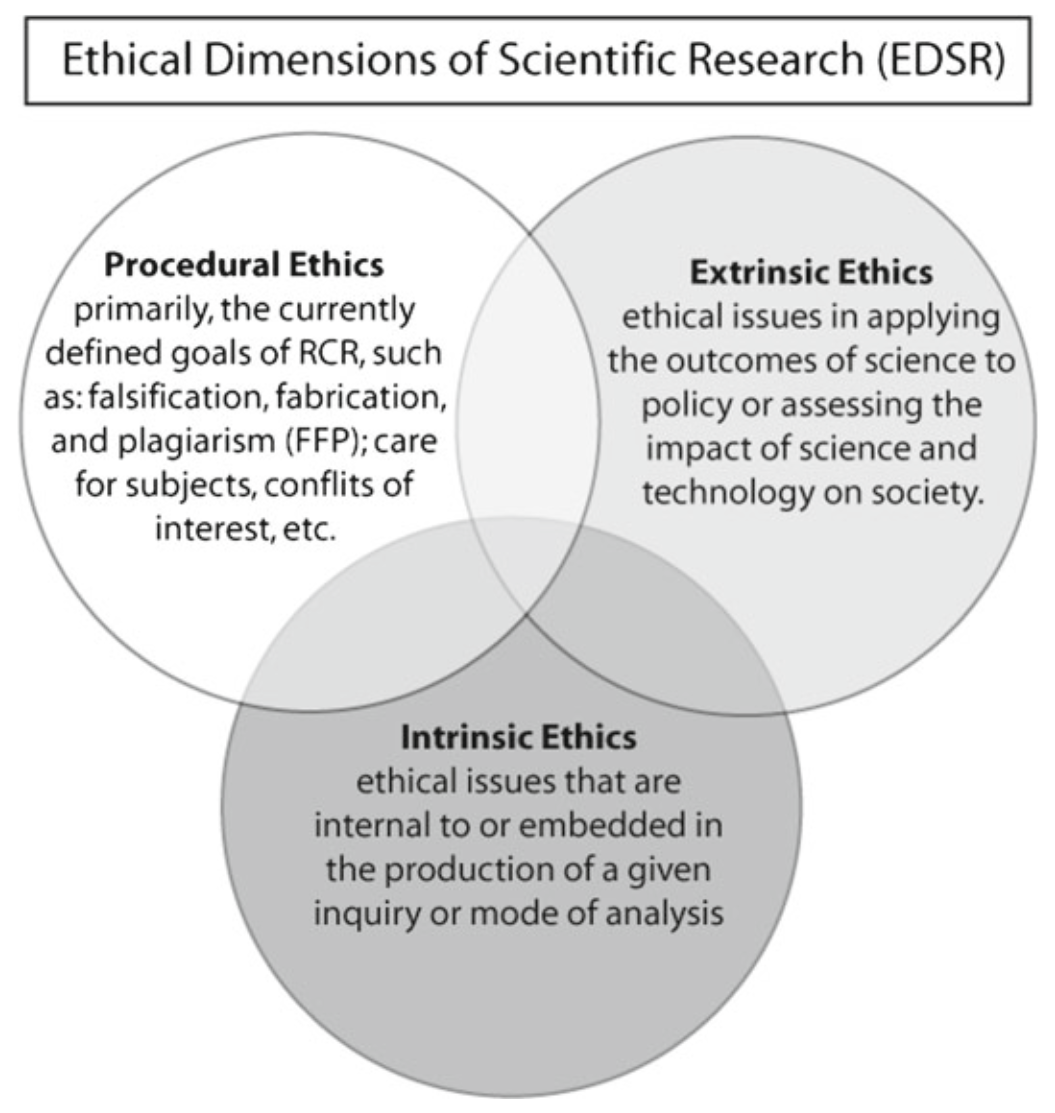
\includegraphics[width=0.6\linewidth]{venn_ethics.png}
    \legende{Les trois dimensions de l'éthique dans la recherche.}{\autocite{tuana_climate_2019} décrit trois dimensions éthiques dans la recherche : l'éthique procédurale consiste en le respect des normes établies et reconnues dans la communauté. C'est en général ce à quoi on fait référence quand on parle de \textit{bonne science}. L'éthique extrinsèque désigne les questions éthiques qui sont liées aux utilisations des productions scientifiques. Enfin, l'éthique intrinsèque désigne les questions qui sont incluses dans le mode de production de la connaissance (en l'occurence, le modèle). }
    \label{fig:diag-venn}
\end{figure}


\subsection{L'éthique procédurale}

L'\gls{procedural ethics} désigne ce qui est couramment regroupé sous le terme de \textit{bonne science}, ou \textit{good science}. Il s'agit de produire de la connaissance en respectant les attentes de la communauté scientifique en termes d'honneteté, de sincérité et de rigueur. Tuana   la définit comme ceci : 

\begin{authoredquote}[\textcite{tuana_leading_2010}, p.479]
Ethical aspects of the process of conducting scientific research, such as: falsification, fabrication, and plagiarism; care for subjects (human and non-human animal); responsible authorship issues; analysis of and care for data.
\end{authoredquote}

La plupart des travaux de modélisation s'inscrivent pleinement dans cette démarche, et sont en phase avec les attentes et bonnes pratiques de la communauté : 

\begin{itemize}
    \item tranparence : les codes sources sont ouverts et accessible, il y a une documentation plus ou moins complète
    \item honneteté : les hypothèses sont clairement énoncées
    \item sincérité des résultats : les résultats sont reproductibles facilement
\end{itemize}

Pourtant, de nombreuses critiques viennent compromettre ce constat. Par exemple, le GIEC remarque qu'il faudrait des explications plus détaillées sur le fonctionnement interne des modèles. 


\begin{authoredquote}[\textcite{noauthor_mitigation_nodate}, p.304]
Transparency is needed to reveal conditionality of results on specific choices in terms of assumptions (e.g., discount rates) and model architecture. More detailed explanations of underlying model dynamics would be critical to increase the understanding of what drives results.
\end{authoredquote}


Un bon exemple est la documentation de FUND. Celle-ci est disponible en ligne, sur le site \href{http://www.fund-model.org/}{fund-model.org/}. Elle est détaillée; toutes les équations et leurs variables y sont décrites; les paramètres en entrée sont également disponibles. De plus, le code source complet, dans un langage open source (julia) est disponible sur github. Il y a donc un véritable effort de transparence et d'ouverture. 

% Pourtant, et comme le remarquent les auteurs de ce modèle, \emph{les modèles sont souvent inutiles dans des mains inexpérimentées}.
Malgré ces efforts importants, il reste difficile de 1/ observer le modèle et en interpréter la conception 2/ le faire tourner pour le réimplémenter.  Par exemple, les paramètres changent de nom, ou ne désignent plus les mêmes choses sans que cela soit indiqué.

Le paramètre $T$, par exemple, désigne successivement \enquote{global mean temperature (in degree centigrade)} et \enquote{global mean temperature above pre-industrial (in degree Celsius) at time t}. Il est plus cohérent avec les equations de considérer qu'il s'agit de la même variable; pourtant, les noms portent à confusion : dans un cas il s'agit d'une valeur mesuré, dans l'autre de l'écart de cette valeur avec la période pré-industrielle. 

Les tables de paramètres sont disponibles aussi, ce qui est beaucoup. Néanmoins, elles sont disponibles sous deux formes peu exploitables. La première est sous une forme de distribution de ces paramètres. Celle-ci a l'avantage de bien comprendre comment ces paramètres sont produits. Néanmoins, sans graine aléatoire, on ne peut pas reproduire à l'identique le fonctionnement du modèle, et ainsi s'assurer que les effets observés ne sont pas simplement liés à un tirage différent. De plus, les distributions sont données en fragments de code Julia, ce qui limite les exports dans d'autres formats. L'autre forme est en texte sur le site. Cette forme présente l'avantage d'être très facilement lisible par des humains. Néanmoins, il est très difficile d'extraire ces données dans un format compatible avec les outils de modélisation, tels que Python ou VENSIM. Dans notre cas, il a donc fallu réfléchir à un programme permettant de convertir le Markdown en format de données CSV, ce qui est à la fois compliqué et source d'erreurs potentielles. \\

Cet exemple nous offre quelques enseignements. D'abord, la tranpsarence est très difficile. Les modèles sont complexes, avec souvent de nombreuses variables et équations, d'autant plus de paramètres et de sources. Ouvrir de manière convenable un modèle est une action couteuse, qui recquière un investissement en temps et en ressource important, alors même que peu de gens sont demandeurs de l'accès aux modèles. Ensuite, qu'elle n'est pas suffisante : avoir accès aux paramètres ne suffit pas à en comprendre les effets sur le modèle. 

Ainsi, le respect des normes scientifiques en termes d'ouverture, de rigueur et de transparence est souvent mis en avant. Dans le cadre de la partie expérimentale de notre travail, nous avons pu constater que des efforts importants sont consentis par les équipes pour mettre à la disposition du plus grand nombre le plus de ressources possibles.  Il y a donc là une première tension, entre une transparence qui n'est jamais suffisante, mais qui est pourtant demandée, tout en étant en réalité peu utilisées (nous en reparlerons dans le chapitre \ref{chapter:socio}. 

%\begin{tcolorbox}
  %  Mais remarques de Keen sur Nordhaus
%\end{tcolorbox}

\subsection{L'éthique intrinsèque}

L'\gls{intrinsic ethics} va plus loin dans l'exigence. Il s'agit de la dimension éthique qui est directement intégrée dans le processus de recherche : il ne s'agit plus de la forme de la recherche, mais du fond de la recherche. 

\begin{authoredquote}[\textcite{tuana_leading_2010}, p.481]
Ethical issues and values that are embedded in or otherwise internal to the production of scientific research and analysis. These involve ethical issues arising from, for example: the choice of certain equations, constants, and variables; analysis of data; handling of error, and degree of confidence in projections.
\end{authoredquote}

Comme le souligne Tuana, la bonne prise en compte de ces questionnements nécessite d'avoir un accompagnement épistémologique au sein des équipes de recherche, c'est-à-dire de prendre en compte ces enjeux comme partie intégrante du développement du projet : \enquote{the domain of intrinsic ethics will not be fully successful unless it includes the expertise of philosophers of science. It is only when this domain becomes a focus of our field, that the range of relevant issues and their ethical and epistemic significance will be fully appreciated}. 


Un exemple de considération d'éthique intrinsèque est le choix du taux d'actualisation. Comme nous l'avons évoqué plus haut, ce paramètre détermine la préférence accordée aux générations actuelles par rapport aux générations futures. Stern présente cette interrogation en ces termes : 

\begin{authoredquote}[\textcite{stern_economic_2007}, p.143]
Modelling over many decades, regions and possible outcomes demands that we make distributional and ethical judgements systematically and explicitly. Attaching little weight to the future, simply because it is in the future (‘pure time discounting’), would produce low estimates of cost – but if you care little for the future you will not wish to take action on climate change.
\end{authoredquote}

Il y a dans le choix de la valeur du taux d'actualisation un jugement éthique qui est central, d'une part parce qu'il répond à un dilemme important, et d'autre part parce qu'il influence grandement les résultats du modèle. 

Cet exemple est régulièrement abordé dans la littérature. On peut prendre aussi d'autres exemples plus proches de l'approche qui a été développée plus haut, notamment autour des questions d'équité spatiale. 

D'abord, le découpage par région. Les modèles se focalisent sur certaines régions plus que d'autres, sont calibrés sur certaines régions (où il y a par ailleurs des données plus nombreuses et de meilleure qualité), et sont donc bien plus pertinents pour décrire les phénomènes dans certaines régions plus que dans d'autres.  

\begin{figure}[htbp]
    \centering
    \begin{minipage}{0.45\textwidth}
        \centering
        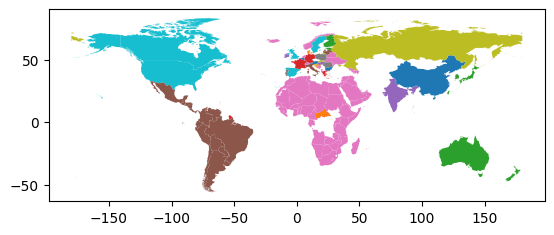
\includegraphics[width=\linewidth]{figures/FUND_regions.png} % Remplacez par le chemin de votre image
        \subcaption{FUND}
        \label{fig:carte_fund}
    \end{minipage}%
    \hfill
    \begin{minipage}{0.45\textwidth}
        \centering
        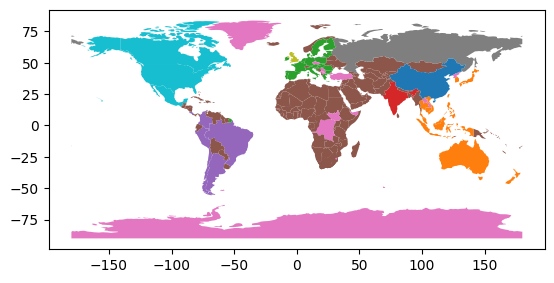
\includegraphics[width=\linewidth]{figures/WILIAM_regions.png} % Remplacez par le chemin de votre image
        \subcaption{WILIAM}
        \label{fig:carte_WILIAM}
    \end{minipage}%
    \legende{Granularité spatiale différente entre les modèles}{}
    \label{fig:trois_cartes}
\end{figure} 

La figure \ref{fig:trois_cartes} montre les différences de régions entre le modèle WILIAM (qui accueille notre expérience) et le modèle FUND. Dans les deux cas, le découpage fait des régions très hétérogènes, qui regroupent elles-mêmes des zones aux caractéristiques différentes. 

Ce double choix de découpage et de granularité est \emph{une} manière \emph{particulière} de décrire le monde, qui résulte d'un contexte social et culturel. Il ne s'agit pas ici de dire qu'il s'agit d'un \emph{mauvais} choix : en effet, ces choix se justifient, et sont d'ailleurs justifié par les équipes de modélisation. WILIAM est un modèle issu du projet LOCOMOTION, financé par l'Union Européenne pour éclairer les décisions de la Commission Europénne \autocite{locomotion-h2020_locomotion-h2020wiliam_model_vensim_2024}. Il donc pertinent qu'il soit centré sur les pays de l'Union Européenne. De la même manière, FUND est particulièrement utilisé par les administrations des Etats-Unis. Il ne s'agit pas non plus de dire que le fait qu'il y ait un choix soit en soit en problème. Bien au contraire, le fait de faire des choix est au coeur de la pratique de la modélisation, et est d'ailleurs ce qui en fait la force. Il s'agit plutôt de mettre en évidence le fait que ces conceptions sont porteuses de valeurs, et qu'elles constituent en cela un enjeu d'éthique intrinsèque. Il faut donc qu'elles soient claires et variées au sein du bouquet de modèles disponibles. 

Un troisième exemple, toujours lié à la question de l'équité spatiale, est celui du pondérateur géographique. L'absence d'un tel pondérateur est, du point de vue du fonctionnement du modèle, équivalente au fait d'avoir un coefficient de 1. Aussi, en en donnant une valeur explicite de 1, puis en faisant varier cette valeur, nous avons cherché à faire apparaitre explicitement dans le modèle ce que nous considérons être une position éthique importante. 

Celle-ci est particulièrement visible dans FUND. L'expression de la valeur d'une vie statistique, dont nous nous sommes inspirés pour produire le pondérateur, est justifiée comme ceci : 

\begin{quote}
    This calibration results in a best guess value of a statistical life that is 200 times per capita income (Cline, 1992). 
\end{quote}

Le choix de la valeur est calibré pour représenter 200 fois le revenu par habitant de la région où il est calculé. La valeur d'une vie est donc : 1/ différente dans chaque région; 2/ proportionnelle au niveau de revenus. Cette approche témoigne de choix éthiques qui ne sont pas négligeables. 

De la même manière, le choix de ne pas pondérer les dommages créés des hiérarchies entre les régions. Des dommages réalisés dans une région 5 fois plus pauvre (au sens du PIB) compteront 5 fois moins que les autres, à dommage égal. Il y a un alignement de la valeur des choses sur leur valeur monétaire. 


\subsection{L'éthique extrinsèque}

Enfin, l'\gls{extrinsic ethics} désigne les questionnements autour des effets de la production scientifique sur la société. C'est une sphère beaucoup plus large, puisqu'elle sort du domaine du laboratoire et de la communauté scientifique, pour mesurer les effets sur les sociétés. 

\begin{authoredquote}[\textcite{tuana_leading_2010}, p.480]
Ethical issues that are external to the production of scientific research. These arise, for example, when considering the impact of scientific research on society; e.g., the effects of technological innovations on social ends such as health and well-being, whether pressing social and economic issues are likely to be addressed and if so, who benefits, and the role of science in policy-making. This domain of ethics also includes ethical concerns arising from the impact of society upon science, for example the impact of funding on research trajectories or the ways in which wide-spread societal biases can impact research trajectories, as they arguably did with eugenics research. In the latter case, there are often links between the domains of extrinsic and intrinsic ethics.
\end{authoredquote}

Ce questionnement s'inscrit dans une réflexion plus large du rapport entre la production scientifique et son application dans la société.  Une conséquence directe est celle qui est liée au cadrage. Comme le montre le GIEC, le cadrage des questions abordées par les modèles intégrés pousse la société dans une direction particulière : 

\begin{authoredquote}[\textcite{intergovernmental_panel_on_climate_change_ipcc_annex_2023}, p.1862]
     IAM analysis could focus on only a subset of relevant futures and thus push society in certain directions without sufficient scrutiny 
\end{authoredquote}

En reprenant l'exemple de l'équité spatiale, les modèles peuvent pousser la société vers un monde où les inégalités de revenu (et leur interaction avec les dommages climatiques) ne sont pas une question (et donc, ni un enjeu ni un problème), voire où elles font partie intégrante d'un monde \emph{optimal}. La notion même de \emph{coût social du carbone} ou de \emph{niveau optimal de changement climatique} intègrent ainsi un niveau \emph{optimal} d'inégalités. En appuyant les politiques publiques et les prises de décisions, ces considérations éthiques dépassent largement le cadre de la science et de ses revues à comité de lecture, où tout un chacun apprécie à leur juste valeur les hypothèses et limites. Au contraire, elles s'invitent discrètement mais totalement à la table des négociations. 

La limite entre l'éthique intrinsèque et extrinsèque peut être tenue, et affaiblit par l'image de certitude que peut vouloir donner la communauté scientifique à l'extérieur. 

\begin{authoredquote}[\textcite{beck_epistemic_2016}, p. 638]
    Hence, the modeling community prefers to discuss controversial modeling issues such as flux adjustments among themselves and to ‘reserve criticism for internal dealings within their own peer community’ (Ref 145, p. 30) because acknowledging uncertainty is seen to make the credibility of climate science in the policy process vulnerable to the attacks of climate skeptics.
\end{authoredquote}

Ce mode de fonctionnement renforce la portée extrinsèque des choix éthiques. En effet, ceux-ci étant masqué, volontairement ou non, aux yeux extérieurs à la communauté, ils sont inscrits pleinement par la manière dont la communauté les montre. 

 Ces considérations sur l'éthique extrinsèque prendront plus de sens dans la section suivante, on l'on développera l'idée que la modélisation participe activement au cadrage du débat public, et donc aux choix de futurs possibles. 

\section{Construire / dessiner les futurs possibles}

Cette section montre que le savoir produit par la science est située dans le temps et dans l'espace. Ainsi, il n'est plus positif, mais bien normatif, en ceci qu'il décrit un univers des possibles. 

Un exemple de à quel point le framing peut impacter la connaissance est la classification des pays. Dans le SPM de l'AR5, les parties n'ont pas pu s'accorder sur un type de classification des pays à adopter; finalement toutes les figures et les textes associés ont été rejetées par les gouvernements. On pourrait ici penser que présenter une information ou une autre n'a pas d'importance, tant que celle-ci a été produite dans les normes scientifiques en vigueur. Pourtant, cet exemple montre que les gouvernements considèrent que le choix d'une classification porte en soi un message trop important; reconnaissant alors l'absence de neutralité du contenu scientifique \autocite{edenhofer_mapmakers_2014}. 

Les modèles intégrés sont utilisés comme base scientifique pour les négociations climatiques. Ils permettent notamment de décrire l'espace des possibles, c'est-à-dire l'ensemble des chemins qui peuvent être pris par les sociétés. Cette relation entre le modèle et la prise de décision est décrite par une image très parlante dans \textcite{edenhofer_mapmakers_2014}, où les modélisateurs sont décrits comme des cartographes, et les décideurs comme des navigateurs. Dès lors, le rôle des modélisateurs-cartographe est de décrire l'espace possible, l'ensemble des zones qui sont navigables; et, si possible, les conditions de navigation que l'on peut rencontrer dans ces zones.  En regard de ces nouvelles connaissances, les décideurs-navigateurs doivent décider du cap à suivre aujourd'hui selon la zone de navigation voulue pour demain. Cette distinction très nette entre décideurs et modélisateurs n'est pas sans limitations. L'une d'entre elle est le cadrage, c'est-à-dire la manière dont le débat public est façonné par le cadre qu'on lui donne.  Plusieurs choses influencent ce cadrage. Nous verrons d'abord que le prisme technique et énergétique agrégé de la plupart des modèles représentent ce genre de contraintes, sans questionner les modèles sous-jacents. Nous verrons ensuite que le choix des variables, et notamment la monétarisation des dommages, fait que de nombreuses dynamiques ne sont soit pas prises en compte, soit prises en compte d'une manière que l'on peut questionner. Enfin, nous, aborderons l'idée que la connaissance est socialement construite, en se basant notamment sur les écrits d'Hélène Longino, pour questionner le caractère universel des résultats des modèles. 

\subsection{Un monde homogène, technique et neutre ?}
\label{ss:model-lineaire}

Les relations entre modélisateurs et décideurs s'inscrivent dans ce que \textcite{aykut_gouverner_nodate} nomment le modèle linéaire de l'expertise. Il s'agit de l'idée selon laquelle \enquote{a connaissance précède l’application et le consensus scientifique précède l’action politique}. Le fonctionnement du \gls{regime climatique} suit en effet ce modèle : les chercheurs publient, sont évalués par le GIEC, qui est interprété par le SBSTA, avant de devenir des politiques climatiques basées sur un consensus scientifique. L'exemple du coût social du carbone va aussi en ce sens : les modèles sont développés, puis évalués par le groupe inter-agence pour le coût social du carbone, avant d'être utilisé dans l'évaluation des politiques publiques par les agences fédérales. 

Il y a dès lors une \enquote{séparation radicale entre science et politique : à la science, les faits, les connaissances ; à la politique, les décisions, les valeurs, les croyances}. 


Helene Longino va plus loin dans sa critique de la science neutre en s'inscrivant dans une perspective d'épistémologie néomarxiste. Elle met en avant trois points principaux : les conséquences du progrès technique, qui découle de la science, les travers du réductionnisme, et la possibilité d'une science plus émancipatrice. Cette approche remet les enjeux de rapport de force au cœur de l'épistémologie, et permet d'avoir une lecture politique de la production scientifique. \\

D'abord, elle clame que les dérives du progrès technique sont les inévitables conséquences de la production scientifique.

\begin{authoredquote}[\textcite{longino_science_1990}, p.210]
    One is that the dystopic applications of modern science — the domination of political life by thermonuclear weapons, new particle beam weapons, and other monsters of annihilation; the control of human potentiality through genetic engineering; the proliferation of toxic wastes from science-based technologies; the displacement of human labor by automation — are not a misuse of socially neutral science but the inevitable result of bourgeois science.
\end{authoredquote}

\begin{authoredquote}[\textcite{intergovernmental_panel_on_climate_change_ipcc_annex_2023}, p.1862]
    There are concerns that IAMs are describing transformative change on the level of energy and land use, but are largely silent about the underlying socio-cultural transitions that could imply restructuring of society and institutions.
\end{authoredquote}


\begin{figure}
    \centering
    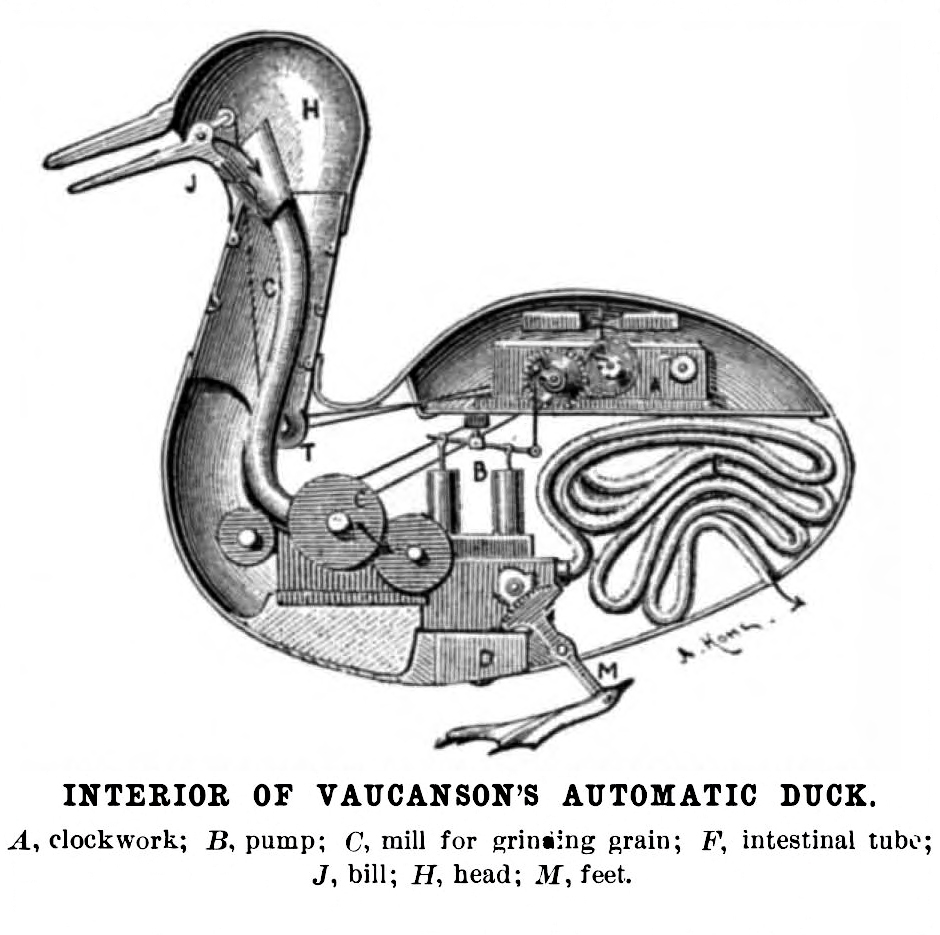
\includegraphics[width=0.6\linewidth]{reductionisme.png}
    \legende{Modèle d'un canard dans une perspective réductioniste}{Le réductionisme tend à décrire les phénomènes par des lois physiques. Les modèles sont des représentations réductionniste du monde.}
    \label{fig:reductionnisme}
\end{figure}



L'autrice continue sa critique en formulant un rejet du réductionnisme, c'est-à-dire à la croyance selon laquelle une notion peut être réduite en d'autres notions plus fondamentales. Elle appelle à une conception plus systémique des relations causales. 

\begin{authoredquote}[\textcite{longino_science_1990}, P.212]
    The spirit, therefore, of these analyses might be better served by seeing them as urging a reconception of objects of inquiry in particular fields — specifically as urging their colleagues to abandon questions presupposing unidirectional or linear causal relations and to understand objects as constituted partly of the parts of which they are wholes and partly of the wholes of which they are parts. If this shift could be accomplished on internalist grounds, there would be less struggle over its acceptance.
\end{authoredquote}

Ce point touche tout à fait les modèles, et particulièrement les fonctions de dommage. Les modèles sont une forme de réductionnisme, puisque l'on représente des phénomènes complexes à travers des fonctions plus simples. Cependant, le fait même de modéliser par des outils de simulation ou d'optimisation impose un réductionnisme, puisqu'il faut réduire les phénomènes complexes et entremêlés à des relations causales directes. Ainsi, cette critique vaut autant dans le cas de modèles très simplificateurs comme DICE, que plus complexes comme FUND.   \\


Une autre difficulté rencontrée par les modèles est la représentation des altérités et des différences. Les modèles tendent à décrire un monde homogène et neutralisé. En effet, les régions sont similaires; elles ont certe des paramétrisations différentes, mais les mécanismes décrits sont les mêmes. On gomme par là les différences culturelles et institutionnelles entre les différentes régions du monde. \\

Ces critiques rejoignent celles formulées par Aykut et Dahan : 

\begin{authoredquote}[\textcite{aykut_gouverner_nodate}, p.19]
    Au cours des années 1990, les pays en développement ne sont convaincus ni de la gravité du risque climatique ni du fait que ce problème les concerne. Ils contestent la prééminence de son traitement « physique » qui privilégie trop, selon eux, le global par rapport au local. Ils critiquent le point de vue de la modélisation numérique globale ou, du moins, le transfert de sa méthodologie au niveau politique ; transfert qui, disent-ils :  
    \begin{itemize}
        \item effacerait le passé (or, le Nord s’est industrialisé, équipé et il a pollué, pas le Sud)
	    \item naturaliserait le présent (en particulier, la référence à l’année 1990 dans le protocole de Kyoto est jugée inacceptable, le présent n’étant pas un acquis, mais devant être interrogé),
	   \item et globaliserait le futur (le CO 2 se globalise sans doute, pas les humains).
    \end{itemize}
\end{authoredquote}

On voit cette homogénéité plus particulièrement lorsqu'elle est questionnée. Le modèle NICE est construit sur le modèle DICE, en prenant en compte des distinctions entre les groupes sociaux, matérialisés par les déciles de revenu \autocite{dennig_inequality_2015}. Les résultats obtenus sont différents de ceux du modèle DICE original; surtout, ils montrent en négatif comment DICE efface ces différences pour en représenter un monde neutre. 

Si cette critique concerne principalement les modèles physiques tels que les modèles de circulation générale, ils peuvent être apportés également aux modèles intégrés. En effet, dans les modèles d'optimisation, où le coût total est minimisé, l'origine des émissions ou le lieu des dommages n'importe pas.  


\subsection{Le cadrage : dans la lumière ou dans l'ombre du projecteur}
\label{ss:cadrage}
% \subsection{La modélisation, une connaissance construite}

Les fonctions de dommage ne peuvent représenter qu'un nombre limité de phénomènes. Par cela, elles cadrent ce que les modèles considèrent comme dommages; si les modèles sont repris dans le débat public ou dans le \gls{regime climatique}, elles cadrent même la perception possible des impacts du changement climatique. \\

\textcite{aykut_gouverner_nodate} donnent cette définition du cadrage (ou \emph{framing} en anglais) : c'est un concept qui  \emph{renvoie à la formulation d’un problème socio-technique dans les discours savants et publics, aux liens établis avec d’autres questions et aux mesures envisagées pour traiter le problème (solutions technologiques ou politiques, approches globales ou locales, etc.), souvent sous-jacentes à son évaluation}. Ils donnent différents éléments permettant de caractériser le cadrage du \gls{regime climatique}. Le premier est sa globalité, c'est à dire l'idée selon laquelle le changement climatique est un problème global, avec des sources globales et des réponses globales. Cette idée prend sa source dans les modèles climatiques, qui, en représentant le climat comme une réalité globale et sans frontières, tendent à effacer les différences locales de responsabilité ou de vulnérabilité. Le cadrage du débat climatique par les sciences du climat se fait par trois canaux principaux : 



\begin{authoredquote}[\textcite{aykut_gouverner_nodate}, p.19]
    \begin{itemize}
    \item la \textbf{concentration sur les modèles globaux de l’atmosphère} comme outil incontournable des projections climatiques, y compris pour les prévisions régionales obtenues par descente en échelle (downscaling) des modèles globaux, a contribué à globaliser les problèmes, à désigner l’arène mondiale/globale comme l’échelle unique de traitement du risque climatique ;
	\item le \textbf{réductionnisme physico-chimique des sciences du climat} tend à mettre en avant les caractéristiques universelles des GES et à les séparer de leur signification sociale locale. Les molécules de méthane des rizières ou celles de gaz carbonique des voitures jouent un rôle identique dans la mise en équation de l’effet de serre. C’est ce que Demeritt (2001) a qualifié de déterminisme environnemental tacite ;
	\item la \textbf{focalisation dans les modélisations sur les « évolutions probables »} a longtemps contribué – contrairement à ce que les critiques récurrentes de « l’alarmisme » des rapports scientifiques suggèrent – à une marginalisation des scénarios du pire et de l’éventualité de changements brusques, ou tipping points. Shackley et Wynne (1996) constatent, dans une étude sur le traitement des incertitudes dans l’expertise climatique globale, une « mise à l’écart des extrêmes » (tuning out of extremes).
\end{itemize}



\end{authoredquote}

Ce cadrage est accentué par les modèles intégrés, en ne permettant le débat que sur les concepts et à partir des hypothèses modélisées. Comme le souligne le GIEC, les modèles intégrés limitent les horizons possibles aux horizons imaginés par les modélisateurs : 

\begin{authoredquote}[\textcite{intergovernmental_panel_on_climate_change_ipcc_annex_2023}]
    IAM analysis could focus on only a subset of relevant futures and thus push society in certain directions without sufficient scrutiny. 
\end{authoredquote}

\begin{authoredquote}[\textcite{intergovernmental_panel_on_climate_change_ipcc_mitigation_2023}, p.304]
    The vast majority of IAM pathways do not consider climate impacts . Equity hinges upon ethical and normative choices. 
\end{authoredquote}

\textcite{cointe_ar6_2024} complète cette remarque en ajoutant que le \emph{corridor} des possibles devient de plus en plus étroit, et limite certaines alternatives, comme des scénarios sans croissance, post-croissance ou de décroissance. 

Plus spécifiquement, les fonctions de dommage peuvent contribuer à cadrer le débat par de nombreux moyens. 

La monétarisation  implique une dichotomie claire entre ce qui est monétaire et ce qui ne l'est pas. Elle ne permet de modéliser que les phénomènes monétaires, et reflète ainsi une importance démesurée des indicateurs économiques classique par rapport à d'autres composantes, tels que le bien-être, la santé ou la biodiversité. Prendre en compte ses différents éléments implique dès lors de les monétariser, ce qui n'est pas sans question. 
De plus, ces modèles vont favoriser des solutions qui s'inscrivent dans le système financier, sans pouvoir proposer d'alternatives. Ainsi, les solutions proposées seront systématiquement des taxes, des coûts du carbone ou d'autres types d'instruments financiers.



\begin{authoredquote}[\textcite{beck_epistemic_2016}, p.630]
    Funtowicz and Ravetz question whether policy-relevant issues can be addressed using conventional scientific techniques ‘when facts are uncertain, values in dispute, stakes high, and decisions urgent.’  In this situation, they claim, a post-normal science that explicitly acknowledges the interweaving of knowledge and ethics is required.
\end{authoredquote}


\subsection{Trouver un niveau optimal de changement climatique, une approche fondamentalement normative}

Une approche à la question du rôle des modèles est celle de la distinction entre les modèles normatifs et positifs. Selon cette catégorisation, très présente en économie, il y aurait d'une part les \emph{sciences économiques}, qui visent à décrire le monde tel qu'il fonctionne, de la manière la plus neutre et précise possible (approche positive). D'autre part, il l'\emph{économie politique} serait plus normative, et viserait à décrire ce que serait un bon fonctionnement de l'économie (approche normative). 

Ainsi, pour Nordhaus \textcite{nordhaus_dice_2013}, \emph{one of the issues that pervades the use of IAMs is whether they should be interpreted as normative or positive}. Selon lui, les modèles de simulation (dont ceux de physique du climat, tels que les modèles de circulation générale) sont positifs, alors que les modèles d'optimisation peuvent être positifs ou normatifs. Par exemple, dans le cas où ils représentent des marchés fonctionnels, ils seraient une représentation précise du fonctionnement de ceux-ci, et donc positifs, tandis qu'ils seraient une approximation correcte du fonctionnement d'autres mécanismes. \\

On peut faire plusieurs critiques sur cette remarque. D'abord, considérer qu'un modèle d'optimisation représente correctement un marché puisque les \emph{mécanismes de marché sont des outils de maximisation ou de minimisation} revient à réduire l'importance de mécanismes non monétaires au sein du fonctionnement des marchés, ce qui est de moins en moins consensuel. 

Ensuite, comme nous l'avons développé plus haut, il est difficile de penser qu'un modèle, même de simulation ou même de sciences du climat, soit neutre. 

Enfin, et si l'on considère que les remarques précédentes sont des critiques inhérentes à tout exercice de modélisation, il convient de remarquer que les modèles d'optimisation sont intrinsèquement normatifs. \\

D'une part, parce qu'en affectant aux dommages une valeur, ils leur confèrent un caractère normatif. Par exemple, affecter à une vie humaine une valeur mobilise un système normatif et des réflexions morales importantes; par ailleurs, ces modèles affectent à différents événements des valeurs différentes. Il y a donc un classement, ou un ordonnancement, qui reflète une hiérarchisation sur une échelle normative. Un argument souvent développé est que le prix dévoile précisément le niveau de préférence, et donc la valeur empirique attribuée par les agents à tel ou tel bien ou service; cependant, ici, les valeurs ne sont pas issues de choix d'agents qui font valoir leurs préférences, mais bien des choix de modélisation. En cherchant à classer, à trouver une solution \emph{optimale}, ces modèles mettent en avant un système normatif particulier. 

D'autre part, parce qu'en contraignant les solutions et les mesures à des valeurs monétaires, ils en font le seul cadre d'analyse possible des effets du changement climatique. En effet, ces modèles valorisent la place d'outils monétaires, qui sont ainsi les seuls à pouvoir être implémentés : taxe carbone, mécanismes de marché, etc. Ainsi, comme le dit \textcite{mercure_modelling_2019}, \emph{the finding that an optimal resource allocation is not achieved due to frictions and market failures, ultimately reflects a normative philosophy of science}. 

\begin{authoredquote}[\textcite{mercure_modelling_2019}]
    This discussion implies that we can interpret optimization models as a device for estimating the equilibrium of a market economy. As such, it does not necessarily have a normative interpretation. Rather, the maximization is an algorithm for finding the outcome of efficient competitive markets.
\end{authoredquote}



\subsection{Prendre en compte le non-monétaire}


\begin{authoredquote}[\textcite{intergovernmental_panel_on_climate_change_ipcc_annex_2023}, p.1844]
    The difficulty in fully representing the extent of climate damages in monetary terms may be the most important and challenging limitation of IAMs and it is mostly directed to costbenefit IAMs. However, all categories of IAMs present important limitations.
\end{authoredquote}




\begin{authoredquote}[\textcite{stern_economic_2007}, p.10]
    First, including direct impacts on the environment and human health (sometimes called ‘non-market’ impacts) increases our estimate of the total cost of climate change on this path from 5\% to 11\% of global per-capita consumption. There are difficult analytical and ethical issues of measurement here. The methods used in this model are fairly conservative in the value they assign to these impacts.  
\end{authoredquote}

Enfin, l'approche néomarxiste fait la promotion d'une science plus émancipatoire, et moins élitiste. Longino évoque notamment les travaux de Hilary Rose et Steven Rose, qui décrivent une science plus émancipatoire, qui aurait \emph{dépassé le clivage entre l'objet et le sujet, entre le rationnel et l'émotionnel, et qui ne serait plus dominée par une rationalité instrumentale. Elle serait caractérisée par des relations sociales démocratiques, c'est-à-dire l'abandon de l'élitisme, et ses théories incorporeraient une vue dialectique de la nature}.


\subsection{L'impossible neutralité des modèles}

Hélène Longino définit deux types de valeurs. D'une part, les \emph{constitutive values}, qui désignent les valeurs méthodologiques admises par la communauté, c'est-à-dire les bonnes pratiques et méthodes. D'autre part, les \emph{contextual values}, qui sont des valeurs personnelles, sociales ou contextuelles des individus. Ces valeurs sont plus normatives, et reflètent le cadre social et culturel dans lequel s'inscrit la démarche scientifique. \\

Se pose dès lors la question du rapport entre ces deux niveaux de valeurs. Dans quelle mesure les valeurs contextuelles influencent les valeurs constitutives, c'est-à-dire dans quelle mesure les normes sociales d'un contexte donné vont influencer la production scientifique ? Et dans quelle mesure les valeurs constitutives influencent les valeurs contextuelles, c'est-à-dire dans quelle mesure la production scientifique influence les normes sociales ? Cette question est celle de l'autonomie de la pratique scientifique du contexte personnel, social et culturel, c'est-à-dire précisément la question de la neutralité de la science. Elle répond de manière très claire à cette question : non seulement les deux interagissent fortement, mais cette interaction est au cœur de la pratique scientifique : 

\begin{authoredquote}[\textcite{longino_science_1990}, p.5]
    I will argue not only that scientific practices and content on the one hand and social needs and values on the other are in dynamic interaction but that the logical and cognitive structuresofscientific inquiry.require such interaction. \textit{p. 5}
\end{authoredquote}

L'autonomie de la production scientifique vis-à-vis des valeurs sociales est donc un mythe. Cependant, et contrairement à ce qui est généralement admis, cela ne remet pas en cause l'intégrité de la recherche. 

\begin{authoredquote}[\textcite{longino_science_1990}]
    Autonomy and integrity are separable attributes, and I shall consider them in sequence.
\end{authoredquote}

La question de la neutralité de la science est régulièrement abordée en épistémologie. Une autrice a particulièrement abordé ce sujet, en montrant que la science est avant tout une pratique sociale, qui s'inscrit dans des dynamiques et un contexte particulier. Il s'agit d'Hélène Longino, dans \emph{Science as social knowledgde} \autocite{longino_science_1990}. Elle développe plusieurs points qui vont être intéressants dans la perspectives des modèles. \\

D'abord, elle développe l'idée que la science n'est pas pure ou dénuée de valeur; au contraire, c'est une base solide pour construire des valeurs ensuite. Il ne s'agit pas de lutter pour une science sans biais ou sans valeur; mais plutot d'inclure ces valeurs au coeur du projet scientifique. 

\begin{authoredquote}[\textcite{longino_science_1990}, p.191]
    Instead of remaining passive with respect to the data and what the data suggest, we can, therefore, acknowledge our ability to affect the course of knowledge and fashion or favor research programs that are consistent with the values and commitments we express in the rest of our lives. From this perspective the idea of a value-free science is not just empty but pernicious. \textit{page 191}
\end{authoredquote}

Elle va ensuite plus loin, en indiquant qu'il y a un choix fort à réaliser, entre s'accorder avec les systèmes normatifs traditionnels, ou s'accorder avec son propre système de valeurs. Le système normatif, qui est forcément inclu dans le processus scientifique, résulte dès lors d'un choix conscient (y compris s'il implique de rester dans le système de valeur traditionnel ou dominant). 

\begin{authoredquote}[\textcite{longino_science_1990}, p.191]
    In particular we can choose between being accountable to the traditional establishment or to our political comrades \textit{p 191}
\end{authoredquote}

Le contexte de la modélisation est particulièrement intéressant de ce point de vue. En effet, comme nous l'avons montré plus haut, les hypothèses sont omniprésentes, et réflètent une conception du monde. Il y a donc un choix réel. Contrairement à ce que certains modélisateurs affirment, il ne s'agit pas d'une réalité objective ou neutre, mais bien d'une sélection hautement normaitve. \\




\cite{helgeson_attention_2022} => pote de Tuana qui parle des valeurs

\section{Responsabilité et doutes normativement inappropriés}

Cette section repose sur les approches des \textit{ignorance studies}, notamment \cite{melo-martin_fight_2018} et \cite{gross_routledge_2015}, avec comme ressources complémentaires \cite{noauthor_carnet_2024} et \cite{proctor_agnotology_2008}. Elle est tirée de réflexions tirées du cours de Mathias Girel à l'ENS \cite{girel_vertus_2023}. 



La question de la responsabilité est épineuse. Nous ne prétendons pas ici établir des conclusions, mais plutôt proposer des outils théoriques susceptibles d'éclairer ce débat. En effet, nous l'avons vu plus haut, la pratique de la modélisation implique d'incorporer des valeurs dans les modèles, et donc de proposer une vision des mondes possibles qui exclue les autres. C'est notamment tout l'enjeu du cadrage (voir \ref{ss:cadrage}). Par ailleurs, et c'est ce que souligne le concept d'éthique extrinsèque, les produits de la modélisation n'engagent pas seulement des réflexions intellectuelles, mais peuvent promouvoir des actions qui ont des répercussions à l'échelle des sociétés, bien en dehors du cadre de la recherche. Deux grandes vues s'opposent quant à la responsabilité des modélisateurs sur ces effets. D'un côté, certains clament qu'en étant rigoureux dans la production scientifique (éthique procédurale), ils sont dans leur exercice normal de production scientifique, et ne sauraient être tenus responsables des conséquences de cette recherche. D'autre, au contraire, dénoncent des résultats parfois considérés comme frauduleux, qui ralentissent l'action climatique et génèrent de ce fait des conséquences adverses et importantes. 

Pour aborder la question de la responsabilité liée au  traitement de l'incertitude, nous nous appuyons sur le concept de doute normativement inapproprié. Il s'agit d'un concept développé par \textcite{melo-martin_fight_2018}, pour tenter de distinguer rigoureusement les doutes légitimes des tentatives de décrédibilisation de la science. 

Ainsi, on oppose au consensus le dissensus. Le consensus correspond à un accord établi par le plus grand nombre, tandis que le dissensus correspond à la remise en question de ce fait accepté. Il y aurait ainsi des dissensus normativement appropriés, qui correspondent aux doutes légitimes qui alimentent la production scientifique et permettent de dépasser des hypothèses toujours imparfaites; et des doutes normativement inappropriés, qui ont pour effet de ralentir la production scientifique sans s'appuyer sur des bases solides \autocite{benalloua_polemique_2023}. 

\paragraph{L'établissement d'une responsabilité}

Pour poursuivre cette réflexion, nous partirons du principe que produire des connaissances qui ont pour finalité de produire de la politique publique créé une forme de responsabilité de la part des chercheurs, en s'alignant sur \textcite{douglas_values_2014, douglas_science_2009} cité par \autocite{beck_epistemic_2016} : 


\begin{authoredquote}[\textcite{beck_epistemic_2016}, p.633]
    Douglas argues that extrinsic ethics (and other non-epistemic consequences of scientific choices) create a specific responsibility for researchers who work on policy-relevant issues with an uncertain evidence base. 
\end{authoredquote}

Cette responsabilité est détaillée un peu plus loin, en précisant les conséquences de l'implémentation des résultats de la recherche. 

\begin{authoredquote}[\textcite{beck_epistemic_2016}, p.633]
     By contrast, the extrinsic ethical consequence of the decision may be the implementation of suboptimal policies with possibly significant societal consequences.
\end{authoredquote}

Ces cas de figure sont parfaitement représentés par les fonctions de dommage, notamment dans les modèles d'optimisation. En effet, des résultats incitant à ralentir ou différer l'action pourraient avoir des conséquences désastreuses s'ils aboutissaient à une mauvaise préparation ou à des choix moins radicaux de réduction des émissions. A l'inverse, une surinterprétation du niveau de dommage pourrait conduire à investir démesurément aujourd'hui, et donc à prioriser les politiques climatiques à d'autres choix de politique budgétaire. 

\paragraph{La fabrique du doute ?}

Ainsi, le doute est nécessaire à la production de connaissances fiables. Nous avons d'ailleurs cherché dans la partie \ref{chapter:modelisation} à remettre en question des hypothèses implicites des modèles, créant ainsi du doute quant aux résultats originels des modèles. De ce point de vue, la diversité des modèles et des opinions est un atout précieux, qui permet de remettre constamment en jeux les résultats et de questionner les hypothèses. Cependant, ces doutes peuvent entrer dans la catégorie des doutes normativement appropriés. \\

Dans son livre \emph{Why are we waiting ?}, Stern développe une réflexion critique sur le rôle des économistes dans la modélisation des impacts du changement climatique \textcite{stern_why_2015}.   En particulier, dans le chapitre \emph{How Some Economic Analyses Have Distorted the Issues}, il s'intéresse à la question des fonctions de dommage dans les modèles intégrés. Il déclare que le rôle central de ceux-ci dans la discussion a fait croire qu'ils représentaient un scénario central.

\begin{authoredquote}[\textcite{stern_why_2015}]
    However, in my view they have played a confusing role in discussions of policy, because the picture most of them have painted is an outlier in the range of possibilities and very far from being a central case. Unfortunately, because the IAMs have been prominent, they have been taken by many, erroneously, as depicting a central case or overall consensus.
\end{authoredquote}

Une sous-section porte un nom encore plus éloquent : \enquote{Impact models: more omissions, overfocus on the tractable, inadequate focus on impacts on lives and livelihoods}. Il y décrit la distance qui se créé entre la modélisation des impacts par les modèles physiques et les représentations qui en sont faites dans les modèles intégrés. \\

Dans un article au titre agressif (\emph{The appallingly bad neoclassical economics of climate change}), l'économiste hétérodoxe Steve Keen produit une critique forte de l'économie du changement climatique, principalement axés autour des travaux de Nordhaus (\textcite{keen_appallingly_2021}). Dès le résumé, il attaque fortement les résultats de ce dernier, en déclarant que \enquote{Nordhaus has misrepresented the scientific literature to justify the using a smooth function to describe the damage to GDP from climate change}, en utilisant \enquote{three spurious methods : assuming that about 90\% of GDP will be unaffected by climate change, because it happens indoors; using the relationship between temperature and GDP today as a proxy for the impact of global warming over time; and using surveys that diluted extreme warnings from scientists with optimistic expectations from economists}. 

Ce papier s'appuie sur de nombreuses références à des articles de Nordhaus et à de la documentation pour mettre en avant des pratiques douteuses pour la production de ces résultats. Les conclusions de Keen sont sans appel; pour lui, Nordhaus est en train de \enquote{drastically underestimating economic damages from global warming}, ce qui en ferait une fausse information majeure ( \enquote{this work could soon be exposed as the most significant and dangerous hoax in the history of science})  et rendraient ces économistes complices (donc en un sens, responsables) des désastres provoqués par le changement climatique (\enquote{these Neoclassical economists will be complicit in causing the greatest crisis, not merely in the history of capitalism, but potentially in the history of life on Earth}).

Ces auteurs pointent du doigt une responsabilité forte des modélisateurs, et Keen va même jusqu'à parler de \enquote{hoax}. 

\paragraph{Une responsabilité, mais pas un NID}

Cependant, ces critiques ne permettent pas forcément de caractériser ces résultats de doute normativement inapproprié. Reprenons ici quelques points issus de \textcite{melo-martin_fight_2018}.

D'abord, la finalité du doute joue un rôle capital. 

\begin{authoredquote}[\textcite{melo-martin_fight_2018}]
    What distinguishes NID from dissent that is merely mistaken is that it fails to yield any of the epistemic benefits that make even false dissent valuable.
\end{authoredquote}

\begin{authoredquote}[\textcite{melo-martin_fight_2018}]
    Hence, we take NID to be not simply dissent that advances incorrect scientific claims but, rather, dissent that fails to promote or that hinders scientific progress.
\end{authoredquote}

Dans le cas des travaux de Nordhaus et des modèles intégrés, il est difficile de prétendre que ce doute n'a pas eu de bénéfice épistémique. En effet, ces travaux ont permis d'intégrer la question climatique dans la réflexion économique (ce qui lui a d'ailleurs valu le Prix dit Nobel d'économie en 2018).  De plus, les nombreux échanges entre Nordhaus et Stern, ainsi que les deux exemples évoqués juste au-dessus montrent comment ces doutes s'inscrivent dans un débat épistémologique. Ainsi, on peut dire qu'en proposant des méthodes, mêmes discutables, ces travaux contribuent à la discussion et ont de ce fait un bénéfice épistémique. \\

Ensuite, une critique pourrait être de mettre en avant les motivations non-épistémiques, et notamment le fait de publier, d'être reconnu, ou de produire des résultats en accord avec les attentes des financeurs des laboratoires. Cependant, le fait qu'il y a des motivations non-épistémiques ne suffit pas à en faire des doutes normativement innapropriés. 

\begin{authoredquote}[\textcite{melo-martin_fight_2018}, p.35]
    But the belief that nonepistemic motivations necessarily result in NID is mistaken. As many have argued, all science, or nearly all science, is in fact unavoidably motivated by some nonepistemic aims.
\end{authoredquote}

Ainsi, les modélisateurs ont une responsabilité épistémique sur les résultats de leurs modèles et leurs applications. 



